\documentclass[a4paper,12pt]{article}

\usepackage[utf8]{inputenc}
\usepackage[MeX]{polski}
\usepackage{fullpage}
\usepackage{graphicx}
\usepackage{hyperref}

\title{\LARGE{[SDPB] Wyznaczanie trasy} \\ \vspace{2mm} \large{Dokumentacja końcowa projektu}}
\author{Michał Aniserowicz, Jakub Turek}
\date{}

\begin{document}
	\maketitle

	\section*{Temat projektu}

	Napisać aplikację wyznaczającą i~porównującą trasę przejazdu na terenie Warszawy środkami komunikacji miejskiej i~samochodem z~opcją ustawienia godziny wyjścia z~domu żeby zdążyć na czas. Aplikacja może być aplikacją mobilną lub przeznaczoną na komputer klasy PC.

	\section*{Założenia}

	Temat został uszczegółowiony poniższymi założeniami:

	\begin{itemize}
		\item Aplikacja zaprojektowana w~architekturze klient-serwer.
		\item Serwer posiada dwie odpowiedzialności:
		\begin{itemize}
			\item Przechowuje dane.
			\item Dostarcza logikę związaną z~przeliczaniem tras.
		\end{itemize}
		\item Klient jest aplikacją dostępową umożliwiającą wprowadzenie następujących danych:
		\begin{itemize}
			\item Lokalizacja początkowa i~docelowa (punkty na mapie).
			\item Docelowy czas przyjazdu.
			\item Przejazd komunikacją miejską lub samochodem.
		\end{itemize}
		\item Klient na wyjściu prezentuje najszybszą trasę dla podanych danych wejściowych oraz godzinę wyjścia/wyjazdu, która pozwala zdążyć na czas.
		\item Dane nie są dostarczane z~systemów zewnętrznych (np. \emph{Google Maps}, \emph{Jak dojadę}), ale składowane w~bazie danych opracowanej w~ramach projektu.
		\item Uproszczenie algorytmu wyznaczania trasy:
		\begin{itemize}
			\item Założenie, że czas przejazdu tego samego odcinka drogi komunikacją miejską i~samochodem jest identyczny.
			\item Brak uwzględnienia informacji o~godzinach przyjazdu środków komunikacji miejskiej na przystanki. Zakłada się, że czas wymagany na przesiadkę jest stały i~jest parametrem algorytmu.
			\item Wyznaczana jest zawsze pojedyncza najszybsza trasa dla wybranego środka komunikacji.
			\item Jako punkt początkowy i~końcowy wybierane są te lokalizacje spośród danych znajdujących się w~bazie, które są najbliższe lokalizacjom wskazanym przez użytkownika.
			\item W~przypadku wskazania komunikacji miejskiej jako środka transportu punktem początkowym i~końcowym podróży są zawsze przystanki najbliższe wskazanym lokalizacjom. Nie jest uwzględniana możliwość dojścia do przystanku.
		\end{itemize}
	\end{itemize}

	\section*{Model danych}

	Tradycyjny, oparty na tabelach model danych nie jest wydajny dla opisu struktury miasta. Struktura ta może być rozpatrywana jako zbiór punktów różnego typu (budynki, skrzyżowania, przystanki autobusowe). Punkty te mogą być ze sobą dowolnie połączone. Połączenie reprezentuje drogę, która umożliwia bezpośrednie przemieszczenie się pomiędzy punktami. Miasto można więc uprościć do przestrzennej struktury grafu planarnego.

	Relacyjny model danych jest problematyczny w~przypadku modelowania relacji wiele-do-wielu. Można wykorzystać dwie strategie:

	\begin{itemize}
		\item Tabela pośrednicząca, która przechowuje mapowanie kluczy obcych w~relacji. Sprawdzanie relacji wymaga wykonania wielu złączeń.
		\item Denormalizacja. Na przykład dla struktury grafowej informację o~wierzchołkach przechowuje się w~tabeli z~krawędziami. W~tym przypadku narzut obliczeniowy na złączenia jest zastępowany narzutem pamięciowym, gdyż każdy wierzchołek jest opisany w~bazie danych $n$ razy, gdzie $n$ to stopień tego wierzchołka.
	\end{itemize}

	Interesującą alternatywę zapewnia ruch \textbf{Not Only SQL}, a~konkretnie jego podzbiór - grafowe bazy danych. Ich wewnętrzny model danych jest spójny z~przedstawioną w~poprzednim akapicie koncepcją opisu struktury miasta. Jednym z~najbardziej dojrzałych projektów grafowych baz danych jest \textbf{Neo4J} (\url{http://www.neo4j.org}). Zaletą tej bazy w~kontekście projektu jest posiadanie warstwy abstrakcji do obliczeń przestrzennych - \textbf{Neo4J Spatial}. Ze względu na wymienione zalety i~odpowiedniość struktury do dziedziny problemu, do implementacji projektu zostanie wykorzystana właśnie baza Neo4J.

	\section*{Architektura aplikacji}

	Aplikacja została zaprojektowana w~architekturze klient-serwer. Szczegółowy schemat architektury przedstawia rysunek~\ref{fig:architecture}. 

	\begin{figure}[ht!]
		\centering
		\scalebox{0.7}[1.0]{
			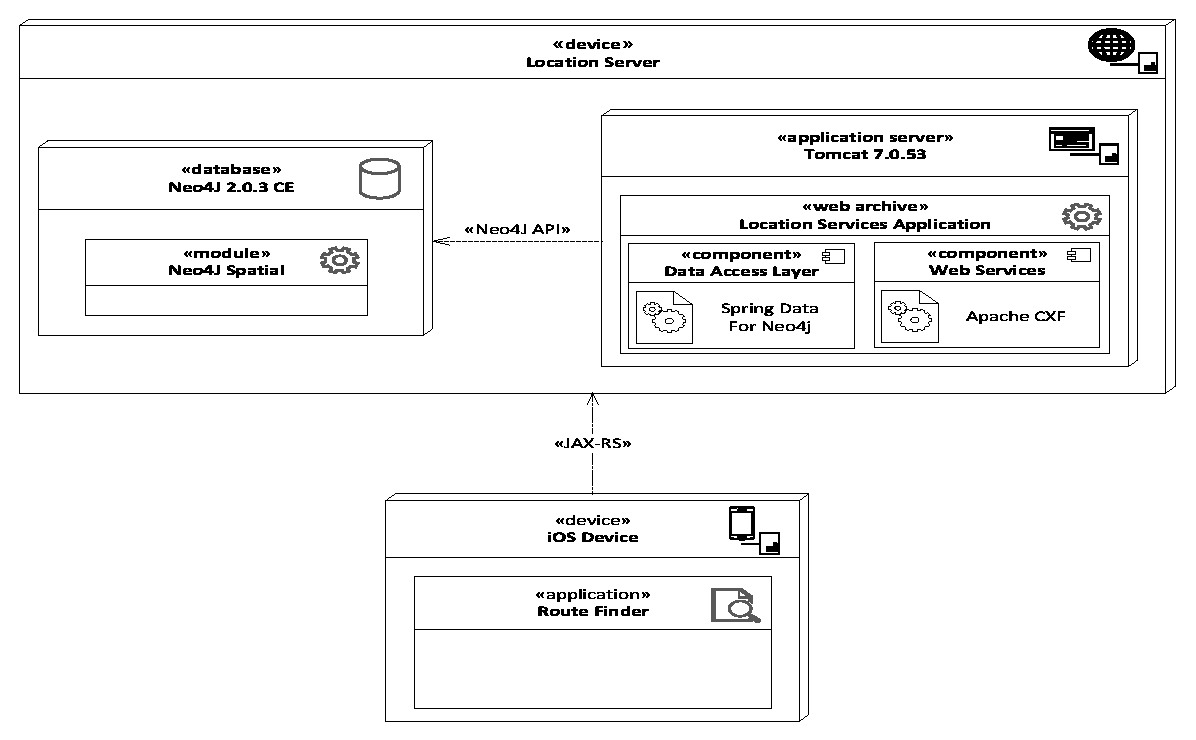
\includegraphics{graphics/architecture.eps}
		}

		\caption{Schemat architektury aplikacji.}
		\label{fig:architecture}
	\end{figure}

\end{document}
